\part{More meshes}
\frame{\partpage}

\begin{frame}{Mesh Formats}
	\begin{itemize}
		\item Typically we invent our own mesh format (see Doom's MD6, Valve's smd formats)
		\pause\item These formats are optimised for realtime rendering and are very efficient
		\pause\item Usually developers write exporters for Maya or 3DSMax to support their format
		\pause\item We are going to use FBX as our model format, this known as an 'interchange' format
	\end{itemize}
\end{frame}

\begin{frame}{Quick Tour of the FBX Format}
	\begin{center}
		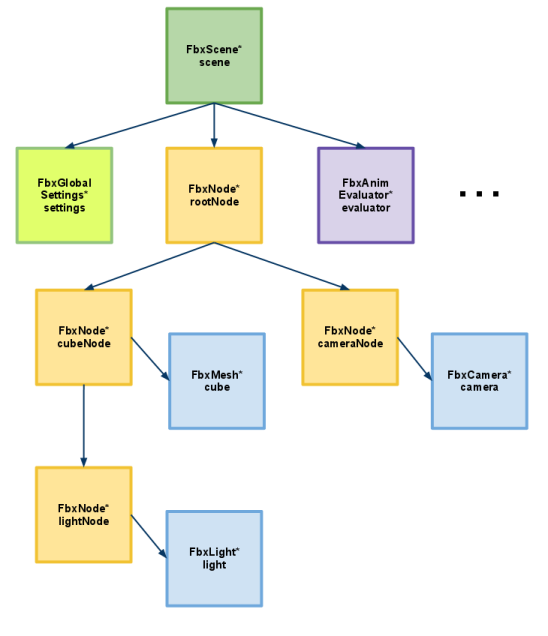
\includegraphics[width=\textwidth,height=0.8\textheight]{scene_org}
	\end{center}
\end{frame}

\begin{frame}{Open Asset Import Library}
	\begin{itemize}
		\item There is an FBX SDK published by Autodesk, this can be used to load FBX files
		\pause\item We will use Asset Import Library to load FBX files
		\pause\item This allows us to support multiple file formats include
		\begin{itemize}
			\pause\item FBX
			\pause\item OBJ 
			\pause\item DAE (aka Collada)
			\pause\item MD5 (DOOM3)
			\pause\item SMD (Half Life 2, Portal etc)
		\end{itemize}
	\end{itemize}
\end{frame}